\documentclass[10pt]{beamer}

\usepackage[utf8]{inputenc}
\usepackage[T1]{fontenc}
\usepackage{amsmath}
\usepackage{graphicx}
\usepackage{tabularx}
\usepackage{array}
\usepackage{booktabs}
\usepackage{tikz}
\usepackage{arydshln}
  \usetikzlibrary{positioning, arrows.meta}

\useoutertheme{miniframes}
\useinnertheme{default}

\definecolor{UHMGreen}{HTML}{024731}
\definecolor{UHMGold}{HTML}{B3995D}
\definecolor{UHMSilver}{HTML}{B2B2B2}
\definecolor{UHMBlack}{HTML}{000000}
\definecolor{UHMWhite}{HTML}{FFFFFF}
\definecolor{Ocean}{HTML}{00758D}
\definecolor{Sky}{HTML}{00A4E2}
\definecolor{Lehua}{HTML}{E3002C}
\definecolor{Ilima}{HTML}{F2A900}
\definecolor{PuaKenikeni}{HTML}{FAD561}
\definecolor{Kukui}{HTML}{D6CBAE}
\definecolor{Akala}{HTML}{E06E8C}
\definecolor{Mao}{HTML}{82B53F}
\definecolor{Lai}{HTML}{00846B}

\setbeamercolor{palette primary}{bg=UHMGreen, fg=UHMWhite}
\setbeamercolor{frametitle}{fg=UHMGreen, bg=UHMWhite}
\setbeamercolor{title}{fg=UHMGreen}
\setbeamercolor{author}{fg=UHMBlack}
\setbeamercolor{institute}{fg=UHMSilver}
\setbeamercolor{date}{fg=UHMSilver}
\setbeamercolor{structure}{fg=UHMGreen} 

\setbeamercolor{section in head/foot}{bg=UHMGreen, fg=UHMWhite!70!UHMSilver}
\setbeamercolor{section in head/foot shaded}{bg=UHMGreen, fg=UHMWhite}

\setbeamerfont{frametitle}{size=\Large, series=\bfseries}
\setbeamerfont{title}{size=\huge, series=\bfseries}
\setbeamerfont{author}{size=\large}
\setbeamerfont{institute}{size=\normalsize}
\setbeamerfont{date}{size=\normalsize}
\setbeamerfont{section in head/foot shaded}{series=\bfseries}

\setbeamertemplate{itemize items}[triangle]
\setbeamercolor{itemize item}{fg=UHMGreen}
\setbeamercolor{enumerate item}{fg=UHMGreen}

\setbeamertemplate{footline}{
  \leavevmode
  \hbox{
  \begin{beamercolorbox}[wd=\paperwidth,ht=2.25ex,dp=1ex]{palette primary}
    \hspace{1em}
    \insertshortauthor
    \hfill
    \insertshortinstitute
    \hfill
    \insertframenumber{}
    \hspace{1em}
  \end{beamercolorbox}}
  \vskip0pt
}

\setbeamertemplate{title page}{
  \vfill
  \begin{center}
    \begin{minipage}{0.9\textwidth}
        \centering
        \usebeamerfont{title}\inserttitle\par
    \end{minipage}
    \bigskip\bigskip
    \vspace{0.5cm}
    \usebeamerfont{author}\insertauthor\par
    \usebeamerfont{institute}Economics 696 - Advanced Topics \\ \insertinstitute\par
    \usebeamerfont{date}\insertdate\par
  \end{center}
  \vfill
}

\newcolumntype{L}[1]{>{\hsize=#1\hsize\raggedright\arraybackslash}X}

\title{The Lame Duck and their Shadows for the Future}
\author[Michael Manolakis]{Michael Manolakis}
\institute[Econ 696 at UH M\=anoa]{University of Hawai`i at M\=anoa}
\date{4th of April 2026}

\begin{document}

\begin{frame}
  \titlepage
\end{frame}



\section{Introduction}

\begin{frame}
    \frametitle{Definition of Lame Duck}
    example \textcolor{Lehua}{more example}.
\end{frame}

\begin{frame}
    \frametitle{Motivation}
    yee haw \\
    \begin{itemize}
        \item oh no
    \end{itemize}
\end{frame}


\begin{frame}
    \frametitle{Research Questions}
      Ze Question?
\end{frame}



\section{Pre stuff}

\begin{frame}
  \frametitle{Pre-Treatment: Measuring Behavioral Types}
  \framesubtitle{Personality Battery}
\end{frame}

\begin{frame}
  \frametitle{Why Not Other Methods}
\end{frame}

\begin{frame}
  \frametitle{Participant Roles and Structure}
  
  At the start of a Treatment, the participant pool is divided:
  \bigskip
  
\end{frame}


\begin{frame}
  \frametitle{The Core Task: The Slider Task}

  \bigskip
  
  \begin{itemize}
    \item \textbf{The Task:} Participants use their mouse to precisely align a series of on-screen sliders within a 90-second time limit.
\end{frame}

\begin{frame}
  \frametitle{The Incentives}

\end{frame}

\begin{frame}
  \frametitle{The Four Experimental Treatments}
  All treatments use an indefinite horizon: there is an 85\% chance the game continues.
\end{frame}

\begin{frame}
  \frametitle{Key Design Choices: Justification (1 of 2)}
  
  \begin{block}{Why an Indefinite Horizon?}
    \begin{itemize}
        \item \textbf{Purpose:} To minimize "end-game effects" where behavior changes near a known final round.
        \item \textbf{Mechanism:} A random continuation probability (Dal Bó, 2005) makes each round feel strategically similar, removing the "pseudo-term limit" of a fixed-length game.
    \end{itemize}
  \end{block}
  
  \begin{block}{Why the "Survivors Only" Rule in T3?}
    \begin{itemize}
        \item \textbf{Purpose:} To create a clean control group for a \textbf{procedurally just} institutional exit.
        \item \textbf{Mechanism:} By focusing only on Representatives who successfully completed their term, to isolate the reaction to a predictable, non-personal removal.
    \end{itemize}
  \end{block}
\end{frame}

\begin{frame}
  \frametitle{Key Design Choices: Justification (2 of 2)}
  
  \begin{block}{Why the Probabilistic Removal (T2b)?}
    \begin{itemize}
        \item \textbf{Purpose:} To achieve clean \textbf{causal identification} of the "betrayal effect."
        \item \textbf{Mechanism:} It creates a group of "unlucky winners" (removed despite voter approval), which separates the effect of injustice from the confound of poor performance.
    \end{itemize}
  \end{block}
  
  \begin{block}{Why the 40\% / 60\% Probabilities?}
    \begin{itemize}
        \item \textbf{Purpose:} To ensure the experiment has sufficient \textbf{statistical power}.
        \item \textbf{Mechanism:} A 40\% chance of an "unlucky winner" makes the key event frequent enough to analyze. The 20-point gap between winning (40\% removal) and losing (60\%) maintains a salient incentive to perform well.
    \end{itemize}
  \end{block}
\end{frame}



\section{Outcomes}

\begin{frame}
  \frametitle{Hypothesis 1: The Procedural Injustice Effect}
  
  \begin{block}{The Core Prediction}
    Unjust, arbitrary removal will trigger significantly more retaliation than a predictable, institutional removal, even when holding performance and voter approval constant.
  \end{block}
  
  \begin{block}{The Test}
    Comparing the sabotage rate of \textbf{"Unlucky Winners"} with the sabotage rate of \textbf{"Term-Limited Survivors"}. Where prediction is:
    \begin{center}
        \textbf{Sabotage Rate (T2b Winners) $>$ Sabotage Rate (T3 Survivors)}
    \end{center}
  \end{block}
  
  \begin{block}{The Alternative (Null Hypothesis)}
    There will be no significant difference in sabotage rates. This would imply that the \textit{procedure} of removal does not matter, only the outcome.
  \end{block}
\end{frame}

\begin{frame}
  \frametitle{Hypothesis 2: Key Comparisons}
  \framesubtitle{The "unlucky winner" effect vs pure betrayal (T2a) and a no-accountability baseline (T1)?}

  \setlength{\leftmargini}{0pt}
  \begin{itemize}
    \item[] \textbf{Pure Betrayal vs. Unlucky Winner:}\\
    \begin{itemize}
      \item The sabotage rate for those purely \textbf{voted out} (T2a) will be high, likely similar to or higher than the "unlucky winners." This establishes the magnitude of the pure betrayal effect. \\
    \end{itemize}
    \item[] \textbf{Accountability vs. No Accountability:}\\
    \begin{itemize}
      \item The sabotage rate for \textbf{Term-Limited Survivors} (T3) will be different from the rate for those removed with \textbf{no voting at all} (T1). This tests if the mere presence of an accountability system alters end-of-term behavior.
    \end{itemize}
    \item[] \textbf{The Alternative (Null Hypothesis)}
    \begin{itemize}
      \item Comparing these treatments will show no difference, implying that neither a pure betrayal nor the presence of accountability has a distinct effect on sabotage rates beyond a simple institutional removal.
    \end{itemize}
  \end{itemize}
  \hspace{2em}
\end{frame}

\begin{frame}
  \frametitle{Hypothesis 3: Heterogeneity by Personality Type}
  \setlength{\leftmargini}{0pt}
    \begin{itemize}
    \item[] \textbf{The Prediction}\\
      The decision to sabotage, particularly in response to a perceived injustice (T2a and T2b), will be driven by stable personality traits. The prediction sabotage will be significantly correlated with pre-treatment measures of:
    \begin{itemize}
      \item Baseline Spite (\texttt{destroy = 1})
      \item Negative Reciprocity (high \texttt{MAO})
    \end{itemize}
    \item[] \textbf{The Test:}\\
    With the use a regression analysis to test if the treatment effects are significantly stronger for individuals with these pre-identified "Power-Seeker" traits.
    \item[] \textbf{The Alternative (Null Hypothesis)}
    \begin{itemize}
      \item Sabotage behavior will be uncorrelated with pre-treatment personality measures, implying the behavior is purely situational and not driven by stable underlying traits.
    \end{itemize}
  \end{itemize}
  \hspace{2em}
\end{frame}






\section{The Theory}

\begin{frame}
  \frametitle{Generalizations}
  \centering 
  \label{tab:generalize}
   \begin{tabularx}{\textwidth}{| L{0.8} | L{1} | L{1.2} |}
    \hline
      \textcolor{UHMGreen}{\textbf{Political Model Component}} & \textcolor{UHMGreen}{\textbf{Generalized Term}} & \textcolor{UHMGreen}{\textbf{Examples in Contexts}} \\
        \hline
        The Representative & The Agent / Incumbent & CEO, fund manager, startup founder, department chair \\
        \hline
        The Voters & The Principal & Board of Directors, limited partners, tenured faculty \\
        \hline
        \textcolor{Lehua}{The ``Power-Seeker''} & Ego-Driven or Status-Motivated & Focused on empire-building \\
        \hline
        \textcolor{Lai}{The ``Public Servant''} & Mission-Driven or Pro-Social & Focused on long-term firm value \\
        \hline
        Sabotage or Retaliation & Costly Post-Termination Externality & Expressed vindication; ex. Poaching key talent \\
        \hline
  \end{tabularx}
\end{frame}

\begin{frame}
    \label{slide:puzzle}
    \frametitle{The Puzzle and Relationship}
    \begin{itemize}
        \item \textcolor{Ocean}{\textbf{Strategic Models}} (Alesina 1990) - Explain debt accumulation to constrain successors. (Rational \& Macro-Level).
        \item \textcolor{Ilima}{\textbf{Behavioral Models}} (Fehr 2006) - Explain reciprocity to unkind acts.
        \item \textcolor{UHMBlack}{\textbf{Missing Link}}: Post-Termination Externalities \\
        Neither explains the specific reaction to the loss of status and the procedural nature of the exit.
    \end{itemize}
    The Core Argument: Proposing that \textcolor{Lehua}{Procedural Injustice} (feeling "betrayed" by voters) triggers latent "Dark Triad" preferences in specific types of leaders. \\
    \hyperlink{slide:dark_triad}{\beamerbutton{Appendix: Dark Triad}}
\end{frame}

\begin{frame}
  \label{slide:Mapping}
  \frametitle{Mapping the Literature: Identifying the Gap} 
  \centering
  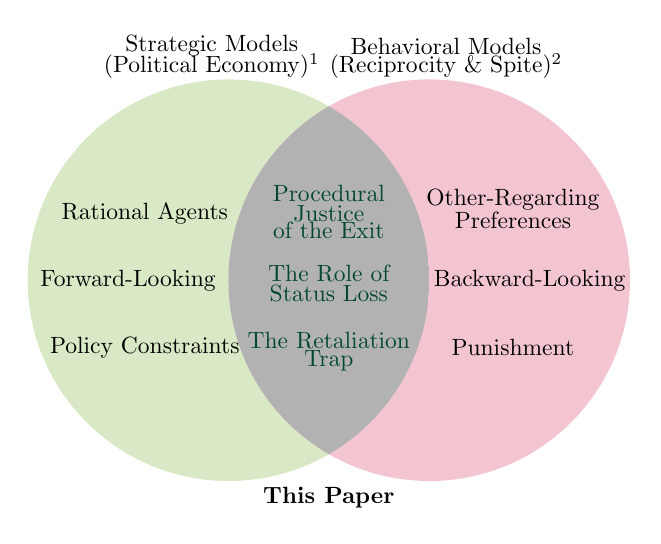
\begin{tikzpicture}[scale=0.85, transform shape]
      % --- Circles ---
      % Draw the two full circles first with their respective colors.
      \fill[Mao!30!white] (0,0) circle (3);
      \fill[Akala!40!white] (3,0) circle (3);

      % --- Intersection ---
      % Use a 'scope' with 'clipping' to isolate the intersection area,
      % then fill it with the desired silver color. This is drawn on top.
      \begin{scope}
          \clip (0,0) circle (3);
          \clip (3,0) circle (3);
          % This fill command only affects the overlapping area
          \fill[UHMSilver] (0,-3) rectangle (3,3);
      \end{scope}

      % --- Text Labels ---
      % Left Circle Text
      \node[align=center] at (-1.25, 1)     {Rational Agents};
      \node[align=center] at (-1.5, 0)      {Forward-Looking};
      \node[align=center] at (-1.25, -1)    {Policy Constraints};
      
      % Right Circle Text
      \node at (4.25, 1.2)                  {Other-Regarding};
      \node at (4.25, 0.9)                  {Preferences};
      \node at (4.5, 0)                     {Backward-Looking};
      \node at (4.25, -1)                   {Punishment};

      % Center Overlap Text (now colored UHMGreen)
      \node[align=center, text=UHMGreen] at (1.5, 1.3)     {Procedural};
      \node[align=center, text=UHMGreen] at (1.5, 1)       {Justice};
      \node[align=center, text=UHMGreen] at (1.5, 0.75)    {of the Exit};
      \node[align=center, text=UHMGreen] at (1.5, 0.1)     {The Role of};
      \node[align=center, text=UHMGreen] at (1.5, -0.2)    {Status Loss};
      \node[align=center, text=UHMGreen] at (1.5, -0.9)    {The Retaliation};
      \node[align=center, text=UHMGreen] at (1.5, -1.2)    {Trap};

      % Outer Text
      \node[align=center] at (1.5, -3.25)   {\textbf{This Paper}};
      \node[align=center] at (-0.25, 3.5)   {Strategic Models};
      \node[align=center] at (-0.25, 3.2)   {(Political Economy)\footnotemark};
      \node[align=center] at (3.25, 3.5)    {Behavioral Models};
      \node[align=center] at (3.25, 3.2)    {(Reciprocity \& Spite)\footnotemark};
  \end{tikzpicture}

  \footnotetext[1]{Alesina (1990), Persson (1989)}
  \footnotetext[2]{Fehr \& Gächter (2000), Zizzo (2001)}
  \hyperlink{slide:alesina}{\beamerbutton{Appendix: To Alesina Models}}
  \hyperlink{slide:games}{\beamerbutton{Appendix: To Related Games}}
  \hyperlink{slide:cost}{\beamerbutton{Appendix: Costly Punishment}}
\end{frame}

\begin{frame}
    \frametitle{The Setting (The Model Environment)}
    The Players:
    \begin{itemize}
        \item Voters (Principal): Risk-averse, want to maximize collective good.
        \item Representative (Agent): Private information on Type $\tau \in \{Good, Bad\}$.
    \end{itemize}
    The Types:
    \begin{itemize}
      \item \textcolor{Lai}{Good (Public Servant): Low cost of effort, pro-social.}
      \item \textcolor{Lehua}{Bad (Power-Seeker): High cost of effort, "Dark Triad" traits (Narcissism), high utility from retaliation.}
    \end{itemize}
    The Timeline:
    \begin{enumerate}
        \item Performance: Rep exerts effort $\to$ Signal $s_t$ observed.
        \item Election: Voters update beliefs $\to$ Retain or Remove.
        \item Legacy (The Twist): If removed, Rep chooses {\textcolor{Lehua}{Sabotage}, Neutral, \textcolor{Lai}{Help}}.
    \end{enumerate}
\end{frame}

\begin{frame}
    \frametitle{The Agent's Utility: The Engine of Retaliation}

    The decision to Sabotage is driven by the agent's utility from their terminal action $a$, given the removal mechanism $k$ and their type $\tau$: 
        {\large \[ U_R(a \mid k, \tau) = W - C(a) + \textcolor{Ilima}{\psi(a, k, \tau)} \]}

    \begin{block}{Breaking it Down}
        \begin{itemize}
            \item \textbf{W:} Final wealth (constant).
            \item \textbf{C(a):} The direct cost of the action (parameter $c$). This is the \textcolor{Lehua}{\textbf{Price of Retaliation}}.
            \item \textbf{$\psi(a, k, \tau)$:} The \textcolor{Ilima}{\textbf{Psychological Utility}}. This is the core behavioral component. Lets assume:
            \begin{itemize}
                \item \textcolor{Lehua}{$\psi(\text{Sabotage} \mid \text{Unjust, Bad}) > 0$}
                \item $\psi$ is zero or negative in all other cases.
            \end{itemize}
        \end{itemize}
    \end{block}
\end{frame}

\begin{frame}
    \frametitle{The Principal's Dilemma: The Retaliation Trap}

        The Principal will \textbf{Fire} a suspected 'Bad' Agent only if: 
          {\large \[ E[U(\text{New Agent})] > E[U(\text{Bad Agent})] + \textcolor{Lehua}{E[\text{Legacy Cost}]} \]}

    \begin{block}{Definition}
        \begin{itemize}
            \item \textcolor{Lehua}{\textbf{E[Legacy Cost]:}} The expected damage from sabotage.
        \end{itemize}
    \end{block}

    \begin{block}{Key Insight}
        \begin{itemize}
            \item When the cost of retaliation ($c$) is low, the \textcolor{Lehua}{$E[\text{Legacy Cost}]$} becomes a \textcolor{Lehua}{large negative number}, forcing the Principal to tolerate the 'Bad Agent'.
        \end{itemize}
    \end{block}

\end{frame}

\begin{frame}
  \label{slide:equilibrium}
    \frametitle{Formalizing the Equilibrium Concept}

    The model is solved for a \textbf{Perfect Bayesian Equilibrium (PBE)}, which is a set of strategies and beliefs where:

    \begin{enumerate}
        \item \textbf{The Representative's Strategy} ($e_t^*(\tau)$) is optimal for each type, given their beliefs about the Voters' removal rule.
        \begin{itemize}
            \item This strategy balances the immediate cost of effort against the future benefit of remaining in office.
        \end{itemize}

        \item \textbf{The Voters' Strategy} (a removal rule) is optimal, given their beliefs ($p_t$) about the Representative's type.
        \begin{itemize}
            \item This rule balances the benefit of removing a suspected 'Bad' type against the risk of incurring the $E[\text{Legacy Cost}]$.
        \end{itemize}

        \item \textbf{Voters' Beliefs} ($p_t$) are formed using \textbf{Bayes' Rule} and are consistent with the Representative's strategy.
    \end{enumerate}
    \hyperlink{slide:bayes}{\beamerbutton{Appendix: Bayes' Rule}} 
\end{frame}

\begin{frame}
  \frametitle{Connecting Theory to Experiment}
  \begin{tabularx}{\textwidth}{| L{1} | L{1} |}
    \hline
    In the Theoretical Model & In the Laboratory Experiment \\
    \hline
    Effort (`$e_t$`) is an \textbf{unobservable choice}. & Effort is the real work of completing the \textbf{Slider Task}. \\
    \hdashline
    It produces a \textbf{noisy signal} of performance (`$s_t$`). &  It is personally costly to the Agent. \\
    \hdashline
    It is personally costly (time, focus). & It produces a \textbf{perfectly observable score} (`slider\_score`\footnote{\alert{The experimental `slider\_score` serves as the clean, measurable proxy for the theoretical concept of effort.}}). \\
    \hline
  \end{tabularx}
\end{frame}



\section{Contributions}
\begin{frame}
  \frametitle{A New Theory of Weak Accountability}
  \framesubtitle{Contribution 1}
  
  \begin{block}{The Conventional View}
    Weak accountability is often attributed to factors like voter apathy, high transaction costs of removal, or a lack of better alternatives.
  \end{block}
  
  \begin{block}{Behavioral Explanation: The "Retaliation Trap"}
    To introduce a more behaviorally-grounded mechanism: rational \textbf{fear}. The hopeful model formalizes how a Principal can become "held hostage" by a credible threat of a spiteful backlash from a removed Agent.
  \end{block}
  
  \begin{block}{The Contribution}
    This reframes institutional inertia not just as a problem of indifference, but as a strategic equilibrium driven by the anticipation of negative psychological reactions.
  \end{block}
\end{frame}

\begin{frame}
  \frametitle{A New Way to Measure the Effect}
  \framesubtitle{Contribution 2}
  
  \begin{block}{The Core Empirical Challenge: Selection Bias}
    In the real world, it's impossible to separate a leader's reaction to being fired from the poor performance that caused the firing. We can't tell if they are angry because they were fired, or just an angry person.
  \end{block}
  
  \begin{block}{Methodological Solution: The "Unlucky Winners" Design}
    The probabilistic removal treatment is designed to break this selection problem. By creating a group of leaders who are removed \textit{despite} performing well enough to win the vote, we can hold performance constant by design.
  \end{block}
  
  \begin{block}{The Expected Finding}
    This will provide clean, causal evidence that \textbf{how} a leader is removed (the procedure) is a distinct and powerful driver of their post-tenure behavior, separate from \textbf{why} they were removed (their performance).
  \end{block}

\end{frame}

\begin{frame}
  \frametitle{Broader Implications}
  \framesubtitle{Contribution 3}
  
  \begin{block}{For Policy}
    \textbf{A New Justification for Institutions} \\
    I hope the findings provide a new rationale for institutions that raise the "price of retaliation." Things like executive non-disparagement clauses, "golden parachutes," or a strong free press can be seen as tools to make the threat of sabotage non-credible, thereby protecting the accountability process.
  \end{block}

  \bigskip
  
  \begin{block}{For Generalizability}
    \textbf{Explaining Corporate \& Organizational Inertia} \\
    The "Retaliation Trap" provides a powerful lens to understand why a corporate board might be slow to fire an underperforming but powerful founder-CEO. The fear is not just a messy transition; it is the fear of the Head actively sabotaging the firm by poaching talent, filing lawsuits, or damaging its reputation.
  \end{block}
\end{frame}



\section{Conclusion}

\begin{frame}
    \frametitle{Summary of Findings (Expected)}
    Theoretical Contribution:
    \begin{itemize}
        \item To formalize the "\textcolor{Lehua}{Retaliation Trap}": Low accountability is not just about laziness, but about \textcolor{Lehua}{fear}.
    \end{itemize}
    Policy Implication:
    \begin{itemize}
        \item Institutions (Golden Parachutes, Norms, Laws) that \textcolor{Lai}{raise $c$ (Cost of Retaliation)} are essential for efficient democracy.
        \item They allow voters to fire bad leaders without fear of burning the house down.
    \end{itemize}
    Experimental Goal:
    \begin{itemize}
      \item To provide the first causal evidence that \textbf{\textcolor{Ilima}{how you are fired matters}} as much as why you are fired.
    \end{itemize}
\end{frame}

\begin{frame}
    \frametitle{Contact Information}
    \vfill
    \begin{center}
        \Large
        % Use \href for email links
        \href{mailto:mmanolak@hawaii.edu}{mmanolak@hawaii.edu} \\
        % Use \href for web links
        \href{https://manolakis.work/}{manolakis.work} \\[0.5cm]
        \textbf{Thank you!}
    \end{center}
    \vfill
\end{frame}



% Let's hide it all in the appendix, hopefully it doesn't burst
\appendix
\section[Appendix]{Appendix}

% Appendix: The Voter's Belief Update (Bayes' Rule)
\begin{frame}
  \label{slide:bayes}
  \frametitle{\large Bayes' Rule}
  The Voters update their belief about the probability that the Representative is a 'Good' type ($p_t$) after observing the performance signal ($s_t$) according to Bayes' Rule:
  {\large
    \begin{align*}
      p_t &= P(\tau=\text{Good} \mid s_t) \\
        &= \frac{ P(s_t \mid \tau=\text{Good}) \cdot p_{t-1} }{ P(s_t) }
    \end{align*}
  }
    \begin{block}{Where:}
      \begin{itemize}
        {\small
          \item $p_{t-1}$ is the prior belief.
          
          \item $P(s_t \mid \tau=\text{Good})$ is the likelihood of observing performance $s_t$ given a 'Good' type (who chooses a high effort level $e^*_{\text{Good}}$).
          
          \item $P(s_t)$ is the total probability of observing $s_t$, calculated using the law of total probability over both types:
          \begin{center}
          $P(s_t) = P(s_t \mid \tau=\text{Good})p_{t-1} + P(s_t \mid \tau=\text{Bad})(1-p_{t-1})$
          \end{center}}
      \end{itemize}
    \end{block}
\hyperlink{slide:equilibrium}{\beamerbutton{Back to Equilibrium Concept}} 
\end{frame}

% Appendix: Full Econometric Specification
\begin{frame}
    \frametitle{Appendix: Econometric Specification}
    \label{slide:specification}
    \resizebox{\textwidth}{!}{
    Primary analysis will use a Probit model to estimate the probability of sabotage:
    }
    \resizebox{\textwidth}{!}{
    $P(\text{Sabotage}_i = 1 \mid X) = \Phi(\beta_0 + \beta_1\text{UnluckyWinner}_i + \beta_2\text{TermLimited}_i + \Gamma'\text{Performance}_i + \Delta'\text{Controls}_i + \epsilon_i)$%
    }
    \begin{block}{Where:}
        \begin{itemize}
            \item $\texttt{Sabotage}_i$: {\small Dummy = 1 if Representative $i$ chooses to sabotage.}
            \item $\texttt{UnluckyWinner}_i$: {\small Dummy = 1 for subjects in T2 removed despite winning the vote.}
            \item $\texttt{TermLimited}_i$: {\small Dummy = 1 for subjects in T3 removed by rule.}
                \begin{itemize}
                    \item \textit{\small(The baseline group is T1: No Vote Term)}
                \end{itemize}
            \item $\texttt{Performance}_i$: {\small Vector of performance metrics.}
            \item $\texttt{Controls}_i$: {\small Vector of pre-experimental measures from the \textbf{Personality Battery}.}
        \end{itemize}
    \end{block}
    \begin{block}{Central Hypothesis Test:}
        $H_0: \beta_1 = 0$ vs. $H_a: \beta_1 > 0$. It is expected $\beta_1$ to be positive and significant.
    \end{block}
    \hyperlink{slide:metrics}{\beamerbutton{Back to Identification}} 
\end{frame}

% Appendix: The Dark Triad and Behavioral Predictions
\begin{frame}
  \label{slide:dark_triad}
  \frametitle{\large The "Dark Triad" and Behavioral Predictions}
  
  The "Power-Seeker" type is a composite. The Personality Battery allows us to disentangle the underlying traits and their predicted effects:
  
  \begin{center}
    \scalebox{0.7}{
      \begin{tabularx}{\textwidth}{ L{1} L{1} L{2} L{0} }
        \toprule
        \textbf{Trait} & \textbf{Core Characteristic} & \textbf{Predicted Behavior in Experiment} \\
        \midrule

        \textbf{Narcissism} & 
        Inflated self-view, high ego sensitivity. & 
        \textcolor{Lehua}{\textbf{Strongest reaction to procedural injustice.} Most likely to sabotage as an "Unlucky Winner," as this is a direct narcissistic injury.} \\
        \midrule

        \textbf{Machiavellianism} & 
        Strategic, manipulative, ends-justify-the-means. & 
        \textcolor{Ocean}{\textbf{Most sensitive to costs ($c$) and detection ($p$).} Less likely to engage in "hot" emotional sabotage; may even "Help" if it serves a strategic purpose.} \\
        \midrule

        \textbf{Psychopathy} & 
        Low empathy, impulsivity, weak norm-adherence. & 
        \textcolor{Lehua}{\textbf{Higher baseline rate of antisocial behavior.} More likely to sabotage across \textit{all} treatments, regardless of the mechanism of removal.} \\

        \bottomrule
      \end{tabularx}
    }
  \end{center}
  \hyperlink{slide:puzzle}{\beamerbutton{Back to Puzzle}}
  \hyperlink{slide:hypotheses}{\beamerbutton{Back to Hypotheses}}
\end{frame}

% Appendix: Alesina and Tabellini Model Points
\begin{frame}
  \label{slide:alesina}
  \frametitle{\large Alesina \& Tabellini Model}

  \begin{center}
    \begin{tabularx}{\textwidth}{ L{1} L{1} }
    \scalebox{0.65}{
      \begin{tabularx}{\textwidth}{ L{2} L{1} L{0} }
        Social Planner's Welfare
        \begin{equation*}
          w_i = E_0 \{ \sum_{t=0}^{T} \sigma^t [u(c_t^i) + v(x_t^i) +\alpha_ih(g_t)+(1-\alpha_i)h(f_t)] \}; 1>\sigma>0    
        \end{equation*} \\

        Intertemporal Budget Constraint
        \begin{equation*}
          \sum_{t=0}^{T} \bar{q}_t c_t \leqq \sum_{t=0}^{T}\bar{q}(1 - \tau_t )(1-x_t)
        \end{equation*}
        \\
        \\
        
        Party D's Welfare
        \begin{equation*}
          W^D = E_0 \{ \sum_{t=0}^{T} \sigma^t [u(c_t) + v(x_t) + h(g_t)] \}
        \end{equation*} \\
        \\
        
        Party R's Welfare
        \begin{equation*}
          W^R = E_0 \{ \sum_{t=0}^{T} \sigma^t [u(c_t) + v(x_t) + h(f_t)] \}
        \end{equation*} \\
      \end{tabularx}
    } &
    \scalebox{0.75}{
      \begin{tabularx}{\textwidth}{ L{0.2} L{1.8} }
        & $c_t$ is Private Consumption \\
        & $x_t$ is Private Investment\\
        & $g_t$ is Spendin on Publicg Good 'g'\\
        & $f_t$ is Spending on Public good 'f'\\
        & $\tau_t$ is Tax Rate\\
        & $\sigma$ is Discount Factor\\
        & $\alpha_t$ is The Polical Preference Parameter\\
        & $\bar{q}_t$ is Present Value Price\\
        & $T$ is terminal period\\
      \end{tabularx}
    } 
    \end{tabularx} 
  \end{center}
  \hyperlink{slide:Mapping}{\beamerbutton{Back to Mapping the Literature}}
  \hyperlink{slide:Mapping}{\beamerbutton{Back to Mapping the Literature}}
\end{frame}

\begin{frame}
  \label{slide:cost}
  \frametitle{\large The Foundation of Costly Punishment}
  \begin{itemize}
    \item \textbf{Game}:Public Goods Game with two conditions.
    \item \textbf{"Without Punishment" Condition}: Standard VCM. Result: Cooperation decays to near-zero levels.
    \item \textbf{"With Punishment" Condition}: After the contribution stage, participants could pay a cost to reduce the earnings of other group members.
    \item \textbf{Cost of Punishment}: Paying 1 unit from your earnings could reduce a target's earnings by 3 units.
    \item \textbf{Key Result}: The threat of punishment sustained high levels of cooperation. Punishment was frequently used, especially against low contributors, even in the final period.
  \end{itemize}
  \hyperlink{slide:Mapping}{\beamerbutton{Back to Mapping the Literature}}
\end{frame}

\begin{frame}
  \label{slide:games}
  \frametitle{\large Zizzo \& Oswald (2001): "Money Burning}
  \begin{enumerate}
    \item \textbf{Spiteful Preferences are Common}: Their main finding is that a majority of people (around two-thirds of their subjects) are willing to pay their own money to "burn" (destroy) the money of others. This is a direct measure of spite or "nastiness."
    \item \textbf{It's About Relative Rank and Fairness}: Burning was significantly higher when the target was perceived as having earned their money through luck rather than effort, and when the burner was in a lower-ranked (disadvantaged) position.
    \item \textbf{It's Costly}: Like punishment, this is a revealed preference. People are willing to become objectively poorer to make someone else even poorer.
  \end{enumerate}
  \hyperlink{slide:Mapping}{\beamerbutton{Back to Mapping the Literature}}
\end{frame}


%Appendix - Isolating Procedural Injustice
\begin{frame}
  \label{slide:injustice}
    \frametitle{Isolating Procedural Injustice}

    \centering
    % The scale has been adjusted slightly to ensure the text fits well
    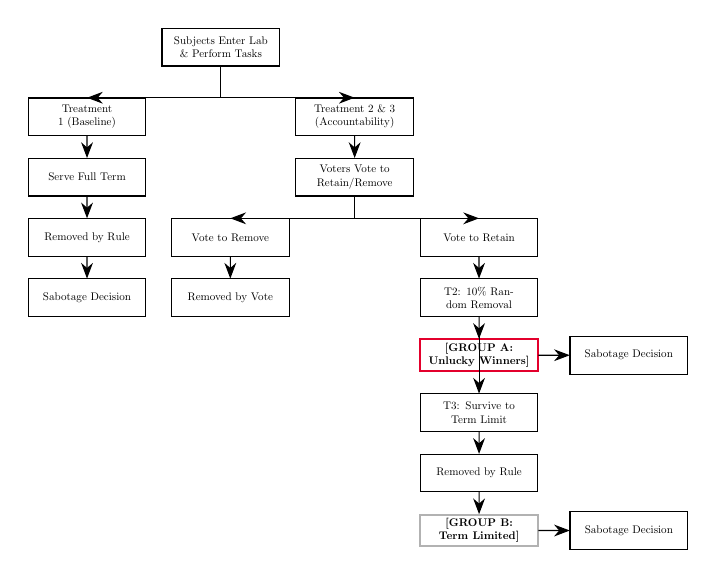
\begin{tikzpicture}[scale=0.4, transform shape,
        node distance = 0.7cm and 1cm, % Vertical and horizontal spacing
        block/.style  = {rectangle, draw, text width=3.5cm, align=center, minimum height=1.2cm},
        % --- MODIFIED STYLES ---
        % Base style for group boxes
        group/.style  = {rectangle, font=\bfseries, align=center, text width=3.5cm},
        % Style for Group A with a thick red border
        group_a/.style= {group, draw=Lehua, thick},
        % Style for Group B with a thick silver border
        group_b/.style= {group, draw=UHMSilver, thick},
        arrow/.style  = {draw, -{Stealth[length=2mm]}} % Style for the arrows
    ]

    \node[block] (start) {Subjects Enter Lab \& Perform Tasks};

    % --- Treatment 1 Branch ---
    \node[block, below left=1cm and 0.5cm of start] (t1) {Treatment 1 (Baseline)};
    \node[block, below=of t1] (t1_serve) {Serve Full Term};
    \node[block, below=of t1_serve] (t1_rule) {Removed by Rule};
    \node[block, below=of t1_rule] (t1_sabo) {Sabotage Decision};

    % --- Treatment 2 & 3 Branch ---
    \node[block, below right=1cm and 0.5cm of start] (t23) {Treatment 2 \& 3 (Accountability)};
    \node[block, below=of t23] (vote) {Voters Vote to Retain/Remove};
    
    % Path A (Vote to Remove)
    \node[block, below left=0.7cm and 0.2cm of vote] (vote_remove) {Vote to Remove};
    \node[block, below=of vote_remove] (removed_by_vote) {Removed by Vote};

    % Path B (Vote to Retain)
    \node[block, below right=0.7cm and 0.2cm of vote] (vote_retain) {Vote to Retain};
    
    % T2 Path
    \node[block, below=of vote_retain] (t2) {T2: 10\% Random Removal};
    % Apply the new 'group_a' style here
    \node[group_a, below=of t2] (group_a) {[GROUP A: Unlucky Winners]};
    \node[block, right=of group_a] (sabo_a) {Sabotage Decision};
    
    % T3 Path
    \node[block, below=of group_a] (t3) {T3: Survive to Term Limit};
    \node[block, below=of t3] (t3_rule) {Removed by Rule};
    % Apply the new 'group_b' style here
    \node[group_b, below=of t3_rule] (group_b) {[GROUP B: Term Limited]};
    \node[block, right=of group_b] (sabo_b) {Sabotage Decision};


    % Arrows
    \draw[arrow] (start.south) |- (t1.north);
    \draw[arrow] (start.south) |- (t23.north);
    
    \draw[arrow] (t1) -- (t1_serve);
    \draw[arrow] (t1_serve) -- (t1_rule);
    \draw[arrow] (t1_rule) -- (t1_sabo);

    \draw[arrow] (t23) -- (vote);
    \draw[arrow] (vote.south) |- (vote_remove.north);
    \draw[arrow] (vote.south) |- (vote_retain.north);
    
    \draw[arrow] (vote_remove) -- (removed_by_vote);
    \draw[arrow] (vote_retain) -- (t2);
    
    \draw[arrow] (t2) -- (group_a);
    \draw[arrow] (group_a) -- (sabo_a);
    
    \draw[arrow] (vote_retain.south) ++(0,-2.5) -| (t3.north);
    \draw[arrow] (t3) -- (t3_rule);
    \draw[arrow] (t3_rule) -- (group_b); 
    \draw[arrow] (group_b) -- (sabo_b);

    \end{tikzpicture}

    % --- COLORED TEXT ---
    \textbf{Core Comparison: Sabotage Rate of \textcolor{Lehua}{GROUP A} vs. \textcolor{UHMBlack}{GROUP B}}
    \hyperlink{slide:params}{\beamerbutton{Back to Experimental Details}} 
\end{frame}

\end{document}